\documentclass[12pt, a4paper]{article}

%<*preamble>
% Math symbols
\usepackage{amsmath, amsthm, amsfonts, amssymb}
\usepackage{accents}
\usepackage{esvect}
\usepackage{mathrsfs}
\usepackage{mathtools}
\mathtoolsset{showonlyrefs}
\usepackage{cmll}
\usepackage{stmaryrd}
\usepackage{physics}
\usepackage[normalem]{ulem}
\usepackage{ebproof}
\usepackage{extarrows}

% Page layout
\usepackage{geometry, a4wide, parskip, fancyhdr}

% Font, encoding, russian support
\usepackage[russian]{babel}
\usepackage[sb]{libertine}
\usepackage{xltxtra}

% Listings
\usepackage{listings}
\lstset{basicstyle=\ttfamily,breaklines=true}
\setmonofont[Scale=MatchLowercase]{JetBrains Mono}

% Miscellaneous
\usepackage{array}
\usepackage{booktabs}\renewcommand{\arraystretch}{1.2}
\usepackage{calc}
\usepackage{caption}
\usepackage{subcaption}
\captionsetup{justification=centering,margin=2cm}
\usepackage{catchfilebetweentags}
\usepackage{enumitem}
\usepackage{etoolbox}
\usepackage{float}
\usepackage{lastpage}
\usepackage{minted}
\usepackage{svg}
\usepackage{wrapfig}
\usepackage{xcolor}
\usepackage[makeroom]{cancel}

\newcolumntype{L}{>{$}l<{$}}
    \newcolumntype{C}{>{$}c<{$}}
\newcolumntype{R}{>{$}r<{$}}

% Footnotes
\usepackage[hang]{footmisc}
\setlength{\footnotemargin}{2mm}
\makeatletter
\def\blfootnote{\gdef\@thefnmark{}\@footnotetext}
\makeatother

% References
\usepackage{hyperref}
\hypersetup{
    colorlinks,
    linkcolor={blue!80!black},
    citecolor={blue!80!black},
    urlcolor={blue!80!black},
}

% tikz
\usepackage{tikz}
\usepackage{tikz-cd}
\usetikzlibrary{arrows.meta}
\usetikzlibrary{decorations.pathmorphing}
\usetikzlibrary{calc}
\usetikzlibrary{patterns}
\usepackage{pgfplots}
\pgfplotsset{width=10cm,compat=1.9}
\newcommand\irregularcircle[2]{% radius, irregularity
    \pgfextra {\pgfmathsetmacro\len{(#1)+rand*(#2)}}
    +(0:\len pt)
    \foreach \a in {10,20,...,350}{
            \pgfextra {\pgfmathsetmacro\len{(#1)+rand*(#2)}}
            -- +(\a:\len pt)
        } -- cycle
}

\providetoggle{useproofs}
\settoggle{useproofs}{false}

\pagestyle{fancy}
\lhead{Лабораторная работа №2}
\lfoot{Михайлов Максим}
\rfoot{M3337}
\cfoot{}
\rhead{стр. \thepage\ из \pageref*{LastPage}}

\newcommand{\R}{\mathbb{R}}
\newcommand{\Q}{\mathbb{Q}}
\newcommand{\Z}{\mathbb{Z}}
\newcommand{\B}{\mathbb{B}}
\newcommand{\N}{\mathbb{N}}
\renewcommand{\Re}{\mathfrak{R}}
\renewcommand{\Im}{\mathfrak{I}}

\newcommand{\const}{\text{const}}
\newcommand{\cond}{\text{cond}}

\newcommand{\teormin}{\textcolor{red}{!}\ }

\DeclareMathOperator*{\xor}{\oplus}
\DeclareMathOperator*{\equ}{\sim}
\DeclareMathOperator{\sign}{\text{sign}}
\DeclareMathOperator{\Sym}{\text{Sym}}
\DeclareMathOperator{\Asym}{\text{Asym}}

\DeclarePairedDelimiter{\ceil}{\lceil}{\rceil}

% godel
\newbox\gnBoxA
\newdimen\gnCornerHgt
\setbox\gnBoxA=\hbox{$\ulcorner$}
\global\gnCornerHgt=\ht\gnBoxA
\newdimen\gnArgHgt
\def\godel #1{%
    \setbox\gnBoxA=\hbox{$#1$}%
    \gnArgHgt=\ht\gnBoxA%
    \ifnum     \gnArgHgt<\gnCornerHgt \gnArgHgt=0pt%
    \else \advance \gnArgHgt by -\gnCornerHgt%
    \fi \raise\gnArgHgt\hbox{$\ulcorner$} \box\gnBoxA %
    \raise\gnArgHgt\hbox{$\urcorner$}}

% \theoremstyle{plain}

\theoremstyle{definition}
\newtheorem{theorem}{Теорема}
\newtheorem*{definition}{Определение}
\newtheorem{axiom}{Аксиома}
\newtheorem*{axiom*}{Аксиома}
\newtheorem{lemma}{Лемма}
\newenvironment{solution}[1][Решение.]{\begin{proof}[#1]}{\end{proof}}

\theoremstyle{remark}
\newtheorem*{remark}{Примечание}
\newtheorem*{exercise}{Упражнение}
\newtheorem{corollary}{Следствие}[theorem]
\newtheorem*{statement}{Утверждение}
\newtheorem*{corollary*}{Следствие}
\newtheorem*{example}{Пример}
\newtheorem{observation}{Наблюдение}
\newtheorem*{prop}{Свойства}
\newtheorem*{obozn}{Обозначение}

% subtheorem
\makeatletter
\newenvironment{subtheorem}[1]{%
    \def\subtheoremcounter{#1}%
    \refstepcounter{#1}%
    \protected@edef\theparentnumber{\csname the#1\endcsname}%
    \setcounter{parentnumber}{\value{#1}}%
    \setcounter{#1}{0}%
    \expandafter\def\csname the#1\endcsname{\theparentnumber.\Alph{#1}}%
    \ignorespaces
}{%
    \setcounter{\subtheoremcounter}{\value{parentnumber}}%
    \ignorespacesafterend
}
\makeatother
\newcounter{parentnumber}

\newtheorem{manualtheoreminner}{Теорема}
\newenvironment{manualtheorem}[1]{%
    \renewcommand\themanualtheoreminner{#1}%
    \manualtheoreminner
}{\endmanualtheoreminner}

\newcommand{\dbltilde}[1]{\accentset{\approx}{#1}}
\newcommand{\intt}{\int\!}

% magical thing that fixes paragraphs
\makeatletter
\patchcmd{\CatchFBT@Fin@l}{\endlinechar\m@ne}{}
{}{\typeout{Unsuccessful patch!}}
\makeatother

\newcommand{\get}[2]{
    \ExecuteMetaData[#1]{#2}
}

\newcommand{\getproof}[2]{
    \iftoggle{useproofs}{\ExecuteMetaData[#1]{#2proof}}{}
}

\newcommand{\getwithproof}[2]{
    \get{#1}{#2}
    \getproof{#1}{#2}
}

\newcommand{\import}[3]{
    \subsection{#1}
    \getwithproof{#2}{#3}
}

\newcommand{\given}[1]{
    Дано выше. (\ref{#1}, стр. \pageref{#1})
}

\renewcommand{\ker}{\text{Ker }}
\newcommand{\im}{\text{Im }}
\renewcommand{\grad}{\text{grad}}
\newcommand{\rg}{\text{rg}}
\newcommand{\defeq}{\stackrel{\text{def}}{=}}
\newcommand{\defeqfor}[1]{\stackrel{\text{def } #1}{=}}
\newcommand{\itemfix}{\leavevmode\makeatletter\makeatother}
\newcommand{\?}{\textcolor{red}{???}}
\renewcommand{\emptyset}{\varnothing}
\newcommand{\longarrow}[1]{\xRightarrow[#1]{\qquad}}
\DeclareMathOperator*{\esup}{\text{ess sup}}
\newcommand\smallO{
    \mathchoice
    {{\scriptstyle\mathcal{O}}}% \displaystyle
    {{\scriptstyle\mathcal{O}}}% \textstyle
    {{\scriptscriptstyle\mathcal{O}}}% \scriptstyle
    {\scalebox{.6}{$\scriptscriptstyle\mathcal{O}$}}%\scriptscriptstyle
}
\renewcommand{\div}{\text{div}\ }
\newcommand{\rot}{\text{rot}\ }
\newcommand{\cov}{\text{cov}}

\makeatletter
\newcommand{\oplabel}[1]{\refstepcounter{equation}(\theequation\ltx@label{#1})}
\makeatother

\newcommand{\symref}[2]{\stackrel{\oplabel{#1}}{#2}}
\newcommand{\symrefeq}[1]{\symref{#1}{=}}

% xrightrightarrows
\makeatletter
\newcommand*{\relrelbarsep}{.386ex}
\newcommand*{\relrelbar}{%
    \mathrel{%
        \mathpalette\@relrelbar\relrelbarsep
    }%
}
\newcommand*{\@relrelbar}[2]{%
    \raise#2\hbox to 0pt{$\m@th#1\relbar$\hss}%
    \lower#2\hbox{$\m@th#1\relbar$}%
}
\providecommand*{\rightrightarrowsfill@}{%
    \arrowfill@\relrelbar\relrelbar\rightrightarrows
}
\providecommand*{\leftleftarrowsfill@}{%
    \arrowfill@\leftleftarrows\relrelbar\relrelbar
}
\providecommand*{\xrightrightarrows}[2][]{%
    \ext@arrow 0359\rightrightarrowsfill@{#1}{#2}%
}
\providecommand*{\xleftleftarrows}[2][]{%
    \ext@arrow 3095\leftleftarrowsfill@{#1}{#2}%
}

\allowdisplaybreaks

\newcommand{\unfinished}{\textcolor{red}{Не дописано}}

% Reproducible pdf builds 
\special{pdf:trailerid [
<00112233445566778899aabbccddeeff>
<00112233445566778899aabbccddeeff>
]}
%</preamble>


\begin{document}

\setcounter{section}{66}

\section{}
Обозначим как $W$ множество всех слов над алфавитом $\{a, b\}$. Объясните равенство $W=Seq\{a\}\times Seq(\{b\}\times Seq\{a\})$. Проверьте равенство производящих функций.

Заметим, что \(Seq(a) = a^*\). Тогда \(Seq\{a\}\times Seq(\{b\}\times Seq\{a\}) = a^* (ba^*)\). Несложно заметить, что искомое верно.

\[
    Seq\{a\}\times Seq(\{b\}\times Seq\{a\}) \leftrightarrow \frac{1}{1 - t} \frac{1}{1 - \frac{t}{1 - t}} = \frac{1}{1 - 2t} \leftrightarrow a_n = 2^n
\]

\section{}
Обозначим как $W^{e}$ множество слов над алфавитом $\{a, b\}$, где все отрезки подряд идущих букв $a$ имеют четную длину. Представьте $W^{e}$ как конструируемый комбинаторный объект. Найдите производящую функцию для $W^{e}$.

\begin{align*}
    Seq \{b\} \times Seq(\{aa\} \times Seq \{b\}) & \leftrightarrow \frac{1}{1 - t}\frac{1}{1 - t^2 \frac{1}{1 - t}} \\
                                                  & = \frac{1}{1 - t - t^2}                                          \\
\end{align*}

\section{}
Обозначим как $W^{(k)}$ множество слов над алфавитом $\{a, b\}$, не содержащих $k$ букв $a$ подряд. Представьте $W^{(k)}$ как конструируемый комбинаторный объект. Найдите производящую функцию для $W^{(k)}$.

\begin{align*}
    Seq \{b\} \times Seq(\{a\} \times Seq_{ < k - 1} \{a\} \times \{a\} \times Seq \{b\} ) & \leftrightarrow \frac{1}{1 - t} \frac{1}{1 - t^2 \frac{1 - t^{k - 1}}{1 - t} \frac{1}{1 - t}} \\
                                                                                           & = \frac{1 - t}{1 + t^2 - 2t - t^2 + t^{k + 1}}                                                \\
                                                                                           & = \frac{1 - t}{1 - 2t + t^{k + 1}}
\end{align*}

\section{}
Постройте производящую функцию для строк над алфавитом $\{a, b\}$, содержащих заданную строку $s$ длины $k$ как подпоследовательность. Сделайте вывод об асимптотическом количестве таких строк.


\[Seq(\{a,b\} \setminus s_1) \times s_1 \times Seq(\{a,b\} \setminus s_2) \times s_2 \dots Seq(\{a,b\} \setminus s_n) \times s_n \times Seq(\{a, b\})\]
\[\left( \frac{t}{1 - t} \right)^k \cdot \frac{1}{1 - 2t}\]
Асимптотически \(\frac{t}{1 - t} \sim 1\), поэтому \(A \sim \frac{1}{1 - 2t}\), т.е. количество строк \(\sim 2^n\), т.е. асимптотически все строки содержат любую подпоследовательность.

% \[
%     Seq\{a\}\times (Seq(\{b\}\times Seq\{a\}) \setminus s) \times s \times (Seq(\{b\}\times Seq\{a\}) \setminus s)
% \]

% \begin{align*}
%     \frac{1}{1 - t} \left(\frac{1}{1 - \frac{t}{1 - t}} - t^k\right) t^k \left(\frac{1}{1 - \frac{t}{1 - t}} - t^k\right) & = \frac{1}{1 - t} \left( \frac{1 - t - t^k(1 - 2t)}{1 - 2t} \right)^2 t^k
% \end{align*}

% \[a_n \sim n \cdot 2^n\]

\section{}
Постройте производящую функцию для строк над алфавитом $\{a, b\}$, в которых нет более $k$ подряд идущих букв $a$ или $b$.

\[Seq_{ < k} \{b\} \times Seq(Seq_{1 \leq, < k} \{a\} \times Seq_{1 \leq, < k} \{b\}) \times Seq_{ < k} \{a\} \]
\begin{align*}
    \frac{1 - t^k}{1 - t} \frac{1}{1 - \left(\frac{t(1 - t^{k - 1})}{1 - t}\right)^2} & = \frac{(1 - t^k)(1 - t)}{(1 - t)^2 - (t - t^k)^2} \\
                                                                                      & = \frac{(1 - t^k)(1 - t)}{(1 - t^k)(1 - 2t + t^k)} \\
                                                                                      & = \frac{1 - t}{1 - 2t + t^k}                       \\
\end{align*}

\section{}
На лекции мы доказали, что если язык регулярный, то производящая функция его слов является рациональной. Докажите или опровергните обратное утверждение: если производящая функция слов языка является рациональной, то язык регулярный.

% Из задачи 121 второго семестра мы знаем, что язык полиндромов над алфавитом мощности \( > 1\) нерегулярен. Найдём производящую функцию для языка палиндромов над алфавитом \(\{a,b \}\).

% \[A_n = \begin{cases}
%         Seq_{n / 2}(2t),       & n\equiv 0\mod 2  \\
%         Seq_{(n + 1) / 2}(2t), & n\equiv 1 \mod 2
%     \end{cases}\]

% \begin{align*}
%     A & = \sum_{n = 0}^{+\infty} A_n                                                \\
%       & = \sum_{n = 0}^{+\infty} A_{2n} + \sum_{n = 0}^{+\infty} A_{2n + 1}         \\
%       & = \sum_{n = 0}^{+\infty} Seq_n(2t) + \sum_{n = 0}^{+\infty} Seq_{n + 1}(2t) \\
%       & = \sum_{n = 0}^{+\infty} (2t)^n + \sum_{n = 0}^{+\infty} (2t)^{n + 1}       \\
%       & = \sum_{n = 0}^{+\infty} (2t)^n + \sum_{n = 0}^{+\infty} (2t)^{n + 1}       \\
% \end{align*}

\section{}
Постройте производящую функцию для строк над алфавитом $\{0, 1\}$, в которых число нулей делится на 3.

Построим ДКА:
\begin{figure}[h]
    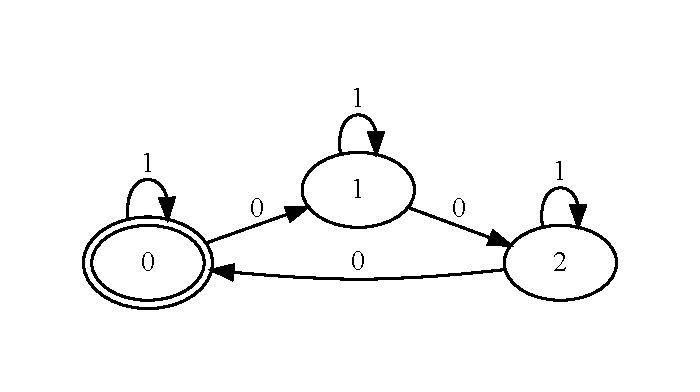
\includegraphics[scale=0.7]{images/73.pdf}
\end{figure}

\[D = \begin{pmatrix} 1 & 1 & 0 \\ 0 & 1 & 1 \\ 1 & 0 & 1 \end{pmatrix} \quad \vec{u} = \begin{pmatrix} 1 & 0 & 0 \end{pmatrix} \quad \vec{v} = \begin{pmatrix} 1 \\ 0 \\ 0 \end{pmatrix}\]

\begin{align*}
    L(t) & = \vec{u}(I - tD)^{ - 1}\vec{v}                                                                                                     \\
         & = \begin{pmatrix} 1 & 0 & 0 \end{pmatrix} \left( \begin{pmatrix} 1 & 0 & 0 \\ 0 & 1 & 0 \\ 0 & 0 & 1 \end{pmatrix} - t  \begin{pmatrix} 1 & 1 & 0 \\ 0 & 1 & 1 \\ 1 & 0 & 1 \end{pmatrix}\right)^{ 1} \begin{pmatrix} 1 \\ 0 \\ 0 \end{pmatrix} \\
         & = \begin{pmatrix} 1 & 0 & 0 \end{pmatrix} \begin{pmatrix} 1 - t & - t & 0 \\ 0 & 1 - t & - t \\ - t & 0 & 1 - t \end{pmatrix}^{ - 1} \begin{pmatrix} 1 \\ 0 \\ 0 \end{pmatrix}                                           \\
         & = \frac{1}{2 t^3 - 3 t^2 + 3 t - 1} \begin{pmatrix} 1 & 0 & 0 \end{pmatrix}
    \begin{pmatrix} -t^2 + 2 t - 1 & t^2 - t        & - t^2          \\
                -t^2           & -t^2 + 2 t - 1 & t^2 - t        \\
                t^2 - t        & -t^2           & -t^2 + 2 t - 1\end{pmatrix}  \begin{pmatrix} 1 \\ 0 \\ 0 \end{pmatrix}                                                                                     \\
         & = \frac{1}{2 t^3 - 3 t^2 + 3 t - 1} \begin{pmatrix} - t^2 + 2t - 1 & t^2 - t & - t^2 \end{pmatrix}
    \begin{pmatrix} 1 \\ 0 \\ 0 \end{pmatrix}                                                                                                                 \\
         & = \frac{- t^2 + 2t - 1}{2 t^3 - 3 t^2 + 3 t - 1}                                                                                    \\
\end{align*}

\section{}
Постройте производящую функцию для строк над алфавитом $\{0, 1\}$, задающие числа в двоичной системе счисления, которые делятся на 3.

Построим ДКА:
\begin{figure}[h]
    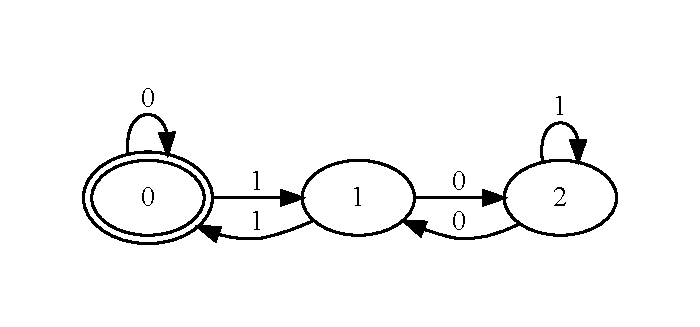
\includegraphics[scale=0.7]{images/74.pdf}
\end{figure}

\[D = \begin{pmatrix}
        1 & 1 & 0 \\
        1 & 0 & 1 \\
        0 & 1 & 1
    \end{pmatrix} \]

\begin{align*}
    (I - tD)^{ - 1} & = \left( \begin{pmatrix} 1 & 0 & 0 \\ 0 & 1 & 0 \\ 0 & 0 & 1 \end{pmatrix} - t \begin{pmatrix}
        1 & 1 & 0 \\
        1 & 0 & 1 \\
        0 & 1 & 1
    \end{pmatrix} \right)^{ - 1} \\
                    & = \begin{pmatrix} 1 - t & - t & 0 \\ - t & 1 & - t \\ 0 & - 1 & 1 - t \end{pmatrix}^{ - 1}                                               \\
                    & = \frac{1}{t^2 + 2 t - 1} \begin{pmatrix}
        (1 - 2 t)/(t - 1) & -t    & t^2/(t - 1)            \\
        -t                & t - 1 & -t                     \\
        t/(t - 1)         & -1    & (-t^2 - t + 1)/(t - 1)
    \end{pmatrix}
\end{align*}

\[\vec{u} (I - tD)^{ - 1} \vec{v} = \frac{1 - 2t}{(t - 1)(t^2 + 2t - 1)}\]

\section{}
Постройте производящую функцию для строк над алфавитом $\{a, b\}$, удовлетворяющих регулярному выражению $(ab|a)^* | (ab|b)^*$

Построим ДКА:
\begin{figure}[h]
    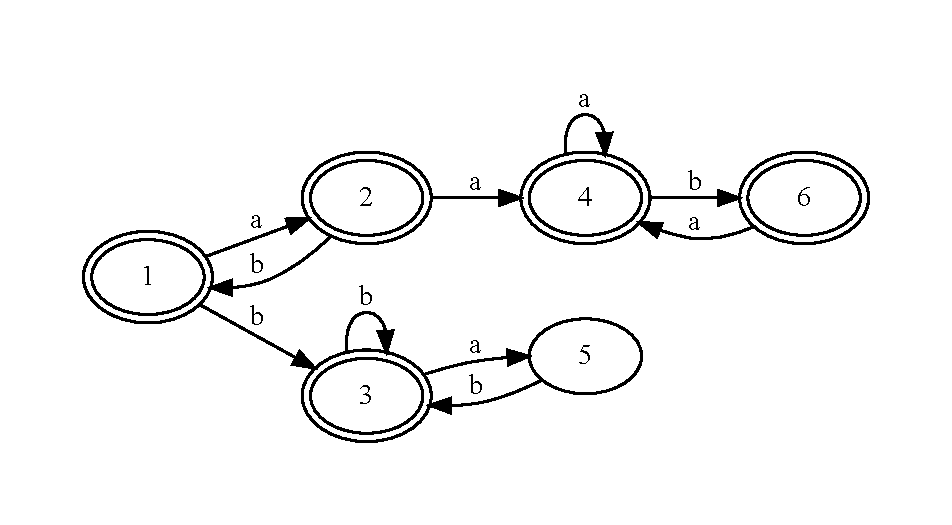
\includegraphics[scale=0.7]{images/75.pdf}
\end{figure}

\[D = \begin{pmatrix}
        0 & 1 & 1 & 0 & 0 & 0 \\
        1 & 0 & 0 & 1 & 0 & 0 \\
        0 & 0 & 1 & 0 & 1 & 0 \\
        0 & 0 & 0 & 1 & 0 & 1 \\
        0 & 0 & 1 & 0 & 0 & 0 \\
        0 & 0 & 0 & 1 & 0 & 0
    \end{pmatrix}\]

\section{}
Найдите производящую функцию для строк, содержащих заданный паттерн $p$ как подстроку.

\(a_n\) = число всех строк - число строк, не содержащих \(p\)

\begin{align*}
    a_n & = b_n - d_n                                          \\
        & = m^n - d_n                                          \\
    A   & = \frac{1}{1 - mt} - \frac{c(t)}{t^k + (1 - mt)c(t)} \\
        & = \frac{t^k}{(1 - mt)(t^k + (1 - mt)c(t))}
\end{align*}

\section{}
Рассмотрим бесконечную случайную строку из $0$ и $1$. Докажите, что матожидание позиции первого вхождения строки $p$ длины $k$ равно $2^k c(\frac 12)$, где $c(z)$ - автокорреляционный многочлен. Указание: можно использовать формулу $\mathbb E X = \sum\limits_{n=0}^{\infty} P(X > n)$.

\begin{align*}
    \mathbb E X & = \sum_{n=0}^\infty P(X > n)                                             \\
                & = \sum_{n=0}^\infty \frac{f(n - k)}{m^{n - k}}                           \\
                & = \sum_{n= k}^\infty \frac{f(n - k)}{m^{n - k}}                          \\
                & = \sum_{n= k}^\infty f(n - k)\cdot t^{n - k}                             \\
                & = \sum_{n= k}^\infty f(n - k)\cdot t^{n - k} \Big|_{t = \frac{1}{m}}     \\
                & = F\left( \frac{1}{m} \right)                                            \\
                & = F\left( \frac{1}{m} \right)                                            \\
                & = \frac{c\left( \frac{1}{m} \right)}{\frac{1}{m^k} + (1 - 1)\cdot \dots} \\
                & = m^k c\left( \frac{1}{m} \right)                                        \\
                & = 2^k c\left( \frac{1}{2} \right)                                        \\
\end{align*}

\section{}
Обозначим как $P^T$ множество разбиений на слагаемые, где порядок слагаемых не важен, а слагаемые выбраны из множества $T$. Осознайте, что $P^T = MSet(Seq_T(Z))$. Найдите производящую функцию для $P^T$.

Осознание очевидно, т.к. \(Seq_T(Z)\) есть множество объектов с весами объектов множества \(T\). Мы можем брать \( > 1\) объект, поэтому \(MSet\)

% \begin{align*}
%     Seq_T(Z)       & = \sum_{t\in T} Seq_t(Z)                                                              \\
%                    & = \sum_{t\in T} \frac{1}{(1 - z)^t}                                                   \\
%     A_n            & = \sum_{t\in T} \binom{t - n - 1}{n}                                                  \\
%     MSet(Seq_T(Z)) & = \prod_{n \geq 1}^{+\infty} \frac{1}{(1 - z^n)^{\sum_{t\in T} \binom{t - n - 1}{n}}} \\
%                    & = \exp \left( \sum_{k \geq 1} \frac{\sum_{t\in T} \frac{1}{(1 - z^k)^t}}{k}  \right)
% \end{align*}

$$Seq_T(Z) \leftrightarrow i\in T$$

$$[n]Seq_T(Z) = \begin{cases}
        0, & n\not\in T \\
        1, & n\in T
    \end{cases}$$

\begin{align*}
    MSet(Seq_T(Z)) & = \prod_{n \geq 1}^{+\infty} \frac{1}{(1 - z^n)^{[n]Seq_T(Z)}} \\
                   & = \prod_{n\in T} \frac{1}{1 - z^n}
\end{align*}

\section{}
Постройте производящие функции для разбиений на различные слагаемые и на нечетные слагаемые. Покажите, что они совпадают.

\begin{align*}
    MSet(\Z /_2) & = \prod_{n = 1}^{+\infty} \frac{1}{1 - z^{2n - 1}}           \\
    PSet(Z)      & = \prod_{n = 1}^{+\infty} (1 + z^n)                          \\
                 & = \prod_{n = 1}^{+\infty} \frac{(1 + z^n)(1 - z^n)}{1 - z^n} \\
                 & = \prod_{n = 1}^{+\infty} \frac{1 - z^{2n}}{1 - z^n}         \\
                 & = \prod_{n = 1}^{+\infty} \frac{1}{1 - z^{2n - 1}}           \\
\end{align*}

\section{}
Постройте производящую функцию для разбиений на не больше, чем $k$ положительных слагаемых.

Будем искать число разбиений на слагаемые из \([1, k]\cap \Z\). Заметим, что это то же самое, т.к. если взять \(m\) раз слагаемое \(n\), то к сумме добавится \(m\cdot n\). Если взять \(n\) раз слагаемое \(m\), то произошло то же самое.

Итого получилась задача 78 для \(T = [1, k]\cap \Z\). Ответ \(\prod_{n = 1}^{k} \frac{1}{1 - z^n}\)

\pagebreak

\section{}
Индекс Хирша. Докажите, что $\prod\limits_{n=1}^\infty\frac{1}{1-z^n}=\sum\limits_{n\ge 1}\frac{z^{n^2}}{((1-z)\cdots(1-z^n))^2}$.

\begin{align*}
    \prod_{n=1}^\infty\frac{1}{1-z^n} & \stackrel{?}{=} \sum_{n\ge 1}\frac{z^{n^2}}{((1-z)\cdots(1-z^n))^2}        \\
                                      & = \sum_{n \geq 1} \left(\prod_{m = 1}^n \frac{1}{1 - z^m}\right)^2 z^{n^2}
\end{align*}

\begin{figure}[h]
    \centering
    \includesvg{images/81.svg}
    \caption{Геометрическое обоснование искомой формулы}
\end{figure}

\end{document}